\DocumentMetadata{}
\documentclass[dvipsnames,12pt]{exam}
% compiles with
% latexmk -pdflatex=lualatex -pdf new.tex

\usepackage[top = 2cm, bottom = 3cm, left=1.5cm, right=1.5cm]{geometry}
\usepackage{microtype}
\usepackage{fontspec}
\usepackage{amssymb}
\usepackage{titlesec}
\usepackage{multicol}
\usepackage{enumitem}
\usepackage{braket}
\usepackage{graphicx}
\usepackage{tikz}
\usepackage{pgfplots}
\usepgfplotslibrary{fillbetween}
\usetikzlibrary{intersections}
\graphicspath{{./img/}}
\usepackage{xcolor}
\usepackage{cancel}
\newcommand\Ccancel[2][black]{\renewcommand\CancelColor{\color{#1}}\cancel{#2}}
\usepackage{amsmath}
\usepackage{hyperref}
\usepackage{eso-pic}
\runningfooter{}{}{\thepage}
\runningheader{}{}{\scriptsize Aayush Bajaj | z5362216}

\hypersetup{
     colorlinks   = true,
     linkcolor    = RedViolet,
     citecolor    = gray
}

\titleformat{\section}{\normalfont\Large\bfseries}{{\color{RedViolet}\S}}{0.5em}{}
\titleformat{\subsection}{\normalfont\large\bfseries}{{\large \color{RedViolet}\S\S}}{0.5em}{}
\titleformat{\subsubsection}{\normalfont\bfseries}{{\color{RedViolet}\S\S\S}}{0.5em}{}

\parindent 0pt
%%% defs courtesy of Denis:
\newcommand{\N}{{\mathbb{N}}}
\newcommand{\C}{{\mathbb{C}}}
\newcommand{\D}{{\mathbb{D}}}
\newcommand{\F}{{\mathcal{F}}}
\renewcommand{\P}{{\mathcal{P}}} %careful with this, it redefines the usual P!
\newcommand{\R}{{\mathbb{R}}}
\newcommand{\Q}{{\mathbb{Q}}}
\newcommand{\T}{{\mathbb{T}}}
\newcommand{\Z}{{\mathbb{Z}}}
\newcommand{\ds}{\displaystyle}
\newcommand{\st}{\,:\,}
\renewcommand{\a}{{\mathbf a}}
\newcommand{\x}{{\mathbf x}}
\newcommand{\y}{{\mathbf y}}
\newcommand{\norm}[1]{\Vert #1 \Vert}
\renewcommand{\mod}[1]{\vert #1 \vert}
\newcommand\vecx{\boldsymbol{x}}
\newcommand\vecy{\boldsymbol{y}}
\newcommand{\zero}{\boldsymbol{0}}
\newcommand{\Arg}{\mathop{\mathrm{Arg}}}
\newcommand{\cl}{\mathop{\mathrm{cl}}}
\renewcommand{\Re}{\mathop{\mathrm{Re}}}
%%% end defs

%% theorems
\usepackage{amsthm}
\newtheorem{theorem}{Theorem}[section]
\newtheorem{corollary}{Corollary}[theorem]
\newtheorem{lemma}[theorem]{Lemma}
\newtheorem{prop}{Proposition}
\newtheorem*{notation}{Notation}

\theoremstyle{definition}
\newtheorem{definition}{Definition}[section]
%%%%%

\AddToShipoutPictureBG*{%  % Note the asterisk (*) - this is important!
  \AtPageCenter{%
    \makebox(0,0){%
      \rotatebox{45}{\textcolor{gray!30}{\fontsize{200}{120}\selectfont FINAL}}%
    }%
  }%
}

\author{Aayush Bajaj | z5362216}
\date{\today}
\title{MATH3611 | Assignment 2}

\begin{document}

\maketitle
\dotfill
\tableofcontents
\vspace{1cm}
\begin{center}

\includegraphics[width=0.2\textwidth]{logo.png}
\end{center}
\vspace{1cm}
\hrule

\newpage

\section{Q1} \label{question1}
Let $(f_n)^\infty_{n=2} \subset C[0,1]$ be a sequence of piecewise linear functions, where $n\in\mathbb{N}$ and $n\geq 2$, and each function $f_n$ is defined by:

$$
    f_n(x) = \begin{cases}
        1, & \text{for } x\in[0,\frac{1}{2}- \frac{1}{n}],\\
        \text{linear}, & \text{for } x\in[\frac{1}{2}-\frac{1}{n}, \frac{1}{2}+\frac{1}{n}],\\
        0, & \text{for } x\in[\frac{1}{2}+ \frac{1}{n}, 1]
    \end{cases}
$$

\begin{enumerate}[label=(\alph*)]
    \item Show that the sequence $(f_n)^\infty_{n=2}$ is Cauchy in the $d_2$ metric, where $$d_2(f,g) = \left ( \int_0^1 | f(x) - g(x) |^2 \,\mathrm{d} x \right )^\frac{1}{2} , f, g \in C[0,1]$$
    \item Show that the sequence $(f_n)^\infty_{n=2}$ is not Cauchy in the $d_\infty$ metric, where $$d_\infty(f,g) = \sup_{x\in[0,1]}|f(x)-g(x)|, f, g \in C[0,1]$$
\end{enumerate}

\begin{definition}\label{definition}
    A sequence $\set{x_n}^\infty_{n=0}$ in a metric space $(X, d)$ is a Cauchy sequence if for every $\epsilon > 0$, there is a $K(\epsilon)$ such that $d(x_m, x_n) < \epsilon$ whenever $m, n > K(\epsilon)$.
\end{definition}

\begin{figure}[ht]
\begin{center}
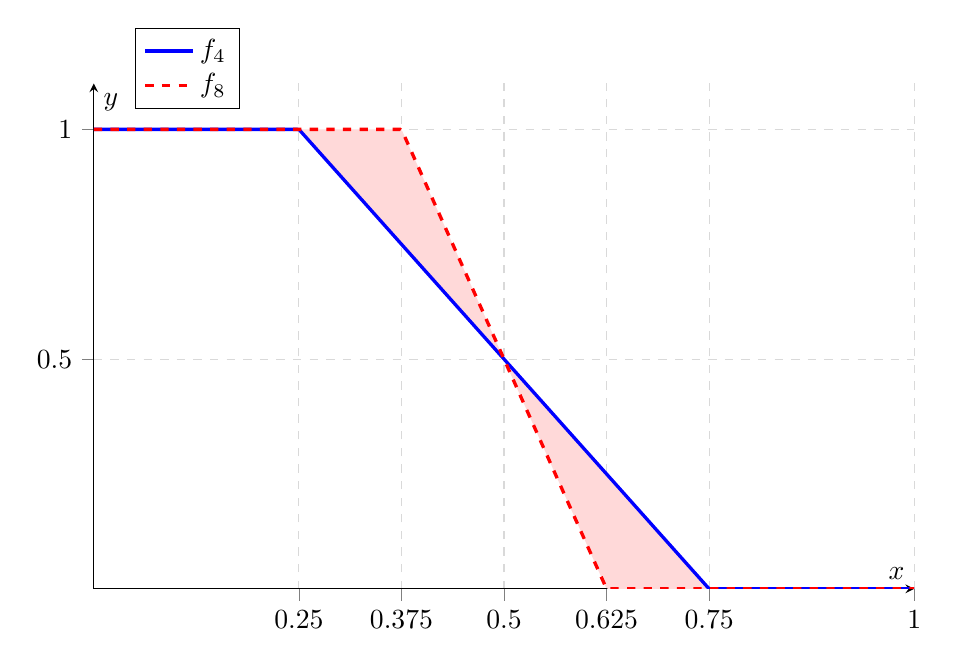
\begin{tikzpicture}
  \begin{axis}[
      axis lines=middle,
      grid = major,
      width=12cm, height=8cm,
      grid style={dashed, gray!30},
      xmin=0, xmax=1,
      ymin=0, ymax=1.1,
      xlabel=$x$,
      ylabel=$y$,
      tick align=outside,
      xtick      ={0,.25,.375,.5,.625,.75,1},
      xticklabels={0,0.25,0.375,0.5,0.625,0.75,1},
      ytick={0,0.5,1},
      legend style={at={(0.05,0.95)},anchor=south west},
      samples=400
    ]

    % f_4
    \addplot[blue,very thick,domain=0:1]
      { x <= 0.25 ? 1 : (x <= 0.75 ? 1 - 2*(x-0.25) : 0) };
    \addlegendentry{$f_{4}$}

    % f_8
    \addplot[red,dashed,very thick,domain=0:1]
      { x <= 0.375 ? 1 : (x <= 0.625 ? 1 - 4*(x-0.375) : 0) };
    \addlegendentry{$f_{8}$}

    \addplot[name path=four,domain=0:1,draw=none]
      { x <= 0.25 ? 1 : (x <= 0.75 ? 1 - 2*(x-0.25) : 0) };
    \addplot[name path=eight,domain=0:1,draw=none]
      { x <= 0.375 ? 1 : (x <= 0.625 ? 1 - 4*(x-0.375) : 0) };
    \addplot[red!15] fill between[
        of=four and eight,
        soft clip={domain=0.25:0.75}
      ];

  \end{axis}
\end{tikzpicture}
    \caption{linear piece-wise for $f_4$ and $f_8$}
\end{center}
\end{figure}

\newpage

\subsection{a)}
\begin{proof}
    For $m > n$\footnote{the same argument applies for $n > m$ by symmetry}:
    \begin{align}
        d_2(f_n, f_m)^2 &= \int^1_0 | f_n(x) - f_m(x) | ^2 \, \mathrm{d}x \\
        &= \int_{I_{m,n}} | f_n(x) - f_m(x) | ^2 \, \mathrm{d}x
    \end{align}
    where $I_{m,n} := [\frac{1}{2}-\frac{1}{n}, \frac{1}{2}+\frac{1}{n}] \cup [\frac{1}{2}-\frac{1}{m}, \frac{1}{2}+\frac{1}{m}]$, i.e. the contributions when $f_n \neq f_m$.\\

    Now, each $f_k$ takes values of 0 and 1 along the flat regions, and remains linear in between: $0 \leq f_k \leq 1$. So $|f_n - f_m |^2 \leq 1$ and we have a bound for the integrand.\\

    Next, by considering the maximal region of integration:
    \begin{align}
        \lambda(I_{m,n}) &= \Ccancel[RedViolet]{\frac{1}{2}}+\frac{1}{n} - (\Ccancel[RedViolet]{\frac{1}{2}}-\frac{1}{n}) + \Ccancel[RedViolet]{\frac{1}{2}}+\frac{1}{m} - (\Ccancel[RedViolet]{\frac{1}{2}}-\frac{1}{m}) \\
        &= \frac{2}{n} + \frac{2}{m} \\
        &< \frac{4}{n}\quad(m > n)
    \end{align}

    We can formulate bounds on our squared metric:
    \begin{equation}
        d_2(f_n, f_m)^2 \leq 1\times \frac{4}{n} \implies d_2(f_n, f_m) \leq \frac{2}{\sqrt{n}}
    \end{equation}
    Fixing $\epsilon > 0$ and $K(\epsilon) := \lceil\frac{8}{\epsilon^2}\rceil$ with $m, n > K(\epsilon)$:
    \begin{equation}
        \frac{2}{\sqrt{n}} < \frac{2}{\sqrt{K(\epsilon)}} < \epsilon
    \end{equation}
    Thus, by the \hyperref[definition]{definition} of a Cauchy sequence, $f_n$ is Cauchy in $(C[0,1], d_2)$.

\end{proof}

\newpage
\subsection{b)}
\begin{proof}
    Contrariwise, we show that there exists an $\epsilon > 0$ such that the \hyperref[definition]{Cauchy condition} fails.

    We accomplish this by picking $m = 2n$ such that 
    \begin{align*}
        z &= \frac{1}{2}-\frac{1}{m}\\
        &= \frac{1}{2}-\frac{1}{2n} \\
        \implies f_m(z) &= 1 \\
        f_n(z) &= \text{linear}
    \end{align*}
    The gradient\footnote{by $\frac{y_2-y_1}{x_2-x_1} = \frac{1-0}{1/2 - 1/n - (1/2 + 1/n)}$} of the linear section is $-\frac{n}{2}$ and the equation for this segment becomes:
    \begin{equation*}
        f_n(z) = 1 - \frac{n}{2}\left(z - \left(\frac{1}{2}-\frac{1}{n}\right)\right) = 1- \frac{n}{2}\left(\frac{1}{n} - \frac{1}{2n}\right) = \frac{3}{4}
    \end{equation*}
    Consequently, $|f_m(z) - f_n(z)| = 1- \frac{3}{4} = \frac{1}{4}$ and
    $$d_\infty(f_n, f_m) = \sup_{x\in[0,1]} |f_n(x) -f_{2n}(x)| \geq \frac{1}{4}$$
    But then with $\epsilon := \frac{1}{8}$ there is \textbf{no} choice of an index $K$ that can satisfy our requirement $d_\infty(f_m, f_n) < \frac{1}{8}$ for $m,n > K(\epsilon)$ because $d_\infty(f_m, f_n)$ is already greater than $\frac{1}{4}$!

    Thus $(f_n)$ is not Cauchy in $(C[0,1],d_\infty)$.
\end{proof}

\newpage
\enlargethispage{1cm}
\section{Question 2}
Show that $\ell^2$ is a vector space; that is, if $x, y \in \ell^2$, then $x + y \in \ell^2$ and $\lambda x \in \ell^2$ for any $\lambda \in \mathbb{R}$. You may assume, without proof, the triangle inequality for the norm $||\cdot||_2$ on $\R^n$ for any $n\in \N$.

\begin{lemma}\label{lemm1}
    \begin{align*}
        (a-b)^2 &\geq 0 \\
        \implies a^2 - 2ab + b^2 &\geq 0 \\
        \implies 2ab &\leq a^2 + b^2 \\
        \implies a^2 + 2ab + b^2 &\leq 2a^2 + 2b^2 \quad\text{ by adding }a^2 + b^2 \text{ to both sides} \\
        \implies (a+b)^2 &\leq 2a^2 + 2b^2
    \end{align*}
\end{lemma}

\begin{lemma}[Triangle Inequality for Absolute Value]\label{lemm2}

    \begin{proof}
    \begin{align*}
        |a+b|^2 &= (a+b)^2 = a^2 + 2ab + b^2 \leq a^2 + 2|ab| + b^2 = (|a| + |b|)^2 \\
        \implies |a+b| &\leq |a| + |b|
    \end{align*}
    \end{proof}
\end{lemma}

\begin{corollary}
    By \ref{lemm1} we have:
    \begin{align*}
        (a+b)^2 &\leq 2a^2 + 2b^2 \\
        \implies (|a|+|b|)^2 &\leq 2|a|^2 + 2|b|^2
    \end{align*}
    Which we can combine with \ref{lemm2}:
    \begin{align*}
        |a + b| &\leq |a| + |b|\\
        |a + b|^2 &\leq (|a| + |b|)^2\\
    \end{align*}
    To produce
    \begin{equation}\label{result1}
        |a + b|^2 \leq (|a| + |b|)^2 \leq 2|a|^2 + 2|b|^2\\
    \end{equation}
\end{corollary}

\begin{notation}
    \begin{align}
        \ell^2 &= \set{\set{x_n}^\infty_{n=1} \subset \R \mid \sum^\infty_{n=1} |x_n|^2 < \infty}\label{l2} \\ 
        \norm{x}_2 &= \left( \sum_{k=1}^\infty |x_k|^2 \right)^{1/2} \label{norm}
    \end{align}
\end{notation}

\newpage
\begin{proof}
    \textbf{Closure under addition:}

    Let $x, y \in \ell^2$ such that $x = \set{x_n}^\infty_{n=1}$ and $y = \set{y_n}^\infty_{n=1}$.

    Then we apply \ref{result1} termwise:
    \begin{align*}
        \sum_{n=1}^\infty |x_n + y_ n |^2 &\leq 2\sum^\infty_{n=1} |x_n|^2 +2\sum^\infty_{n=1}|y_n|^2 \\
        &= 2||x||_2^2 + 2||y||_2^2
    \end{align*}

    By the comparison test, we have found $||x+y||_2^2 \leq 2||x||_2^2+2||y||_2^2$ and we know that $||x||_2^2 + ||y||_2^2$ converges by our assumption of both being in $\ell^2$ and hence being the sum of two finite real numbers.\\

    \textbf{Closure under scalar multiplication:}

    Let $\lambda \in \R$ and $x\in\ell^2$:
    \begin{align*}
        \sum^\infty_{n=1}|\lambda x_n |^2 &= \lambda^2 \sum^\infty_{n=1} |x_n|^2 \\ 
        &= \lambda^2 \norm{x}_2^2
    \end{align*}
    Which is finite because $\norm{x}^2_2 < \infty$. Thus $\lambda x \in \ell^2$.

\end{proof}

\newpage
\section{Question 3}
Show that the subset $c_{00}$ is dense in the metric space $\ell^2$.\footnote{ i.e. we wish to show that for $x\in \ell^2$ and $\epsilon > 0, \; \exists x_\epsilon \in c_{00}$ such that $\norm{x-x_\epsilon}_2 < \epsilon$.}

\begin{proof}
    Let \hyperref[l2]{$\ell^2$} be the space of square-summable sequences equipped with the \hyperref[norm]{2-norm}.\\

    Let $c_{00} = \left\{ \{x_n\}_{n=1}^\infty \in \ell^2 \mid x_n = 0 \text{ for all but finitely many } n \right\}$ be the subset of sequences with only finitely many non-zero terms.\\

    Fix $x = \set{x_n}_{n=1}^\infty \in \ell^2$ and $\epsilon > 0$. Since $x \in \ell^2$, the series $\sum^\infty_{n=1}|x_n|^2$ converges to a finite value. By the definition of convergence for an infinite series\footnote{we can make the tail of the series arbitrarily small. this follows because the partial sums $s_p = \sum_{n=1}^p |x_n|^2$ converge to $S=\norm{x}_2^2$ and the remainder $\sum_{n=p+1}^\infty |x_n|^2 = S - s_p$ can be made arbitrarily small for sufficiently large $p$.
    \[
        \sum^\infty_{n=p+1}|x_n|^2 < \delta
    \]}:
    \[
        \sum^\infty_{n=p+1}|x_n|^2 < \epsilon^2\quad\text{with }\delta\text{ as }\epsilon^2
    \]
    Construct $x_\epsilon = \set{x_n^{(\epsilon)}}^\infty_{n=1} \in c_{00}$ by defining
    \[
    x_n^{(\epsilon)} = \begin{cases} 
        x_n & \text{if } 1 \leq n \leq p, \\
        0 & \text{if } n \geq p + 1.
    \end{cases}
    \]

    Thus, $x_\epsilon = (x_1, x_2, \ldots, x_p, 0, 0, \ldots)$, which has finitely many non-zero terms and belongs to $c_{00}$.

    Computing the difference $x - x_\epsilon = \{x_n - x_n^{(\epsilon)}\}_{n=1}^\infty$ for each index $n$ yields:
    \[
    x_n - x_n^{(\epsilon)} = \begin{cases} 
        x_n - x_n = 0 & \text{if } 1 \leq n \leq p, \\
        x_n - 0 = x_n & \text{if } n \geq p + 1.
    \end{cases}
    \]

    So, $x - x_\epsilon = (0, 0, \ldots, 0, x_{p + 1}, x_{p + 2}, \ldots)$, where the first $p$ terms are zero. Thus the $\ell^2$-norm of the difference becomes
    \[
        \norm{x-x_\epsilon}_2 = \left(\sum_{n=1}^\infty |x_n - x_n^{(\epsilon)}|^2 \right )^\frac{1}{2} = \left( \sum_{n=p+1}^\infty |x_n|^2 \right )^\frac{1}{2} < (\epsilon^2)^\frac{1}{2} = \epsilon,
    \]
    since $\sum_{n=p + 1}^\infty |x_n|^2 < \epsilon^2$ by the choice of $p$.

    In conclusion, for any $x \in \ell^2$ and $\epsilon > 0$, there exists $x_\epsilon \in c_{00}$ such that $\norm{x - x_\epsilon}_2 < \epsilon \implies c_{00}$ is dense in $\ell^2$.

\end{proof}

\end{document}
